


\documentclass[10pt,handout]{beamer}
\setbeamertemplate{navigation symbols}{}
\usefonttheme{serif} 
\usepackage{amsmath}
\usepackage{amssymb}
\usepackage{graphicx}
\usepackage{cite}
\usepackage{color} 
\usepackage{setspace}
\usepackage{hyperref}

\newcommand{\xx}{{\bf{x}}}
\begin{document}
\title{Machine Learning I Lecture IV:\\ Bayesics of Inference}   
\author{Jakob H Macke\\ Max Planck Institute for Biological Cybernetics\\ Bernstein Center for Computational Neuroscience} 
\date{XY.XY.2012} 

\frame{\titlepage} 

\frame{\frametitle{Plan for today}\tableofcontents} 


\section{Bayesian Inference} 
\frame{\frametitle{'Bayesian Inference' refers to computation of the posterior distribution over parameters given the data.} 
\begin{itemize}
\item Data $\mathcal{D}=\{t_1, t_2, \ldots, t_N\}$ \pause
\item Supervised learning: $\mathcal{D}=\{(x_1,t_1), (x_2,t_2), \ldots, (x_N,t_N)\}$ \pause
\item Likelihood function $P(t|w)$ \hspace{1cm}(parameterized by $w$)\pause
\item $P(D|w)= \prod_{n=1}^N P(t_n|w)$\pause
\item Prior distribution $\pi(w)$\pause
\item Bayes rule: $\mbox{Posterior} \propto \mbox{Likelihood}  \times \mbox{Prior}$
\begin{align}
P(w | D) =\frac{1}{Z} P(D|w) P(w)
\end{align}\pause
\item Probabilities must normalize to $1$: 
\begin{align}
Z= P(D)= \int P(D|w) P(w) dw
\end{align}
\end{itemize}

}

%\subsection{Subsection no.1.1  }
%\frame{ 
%Without title somethink is missing. 
%}
\frame[shrink=5]{\frametitle{We can use the posterior distribution to make predictions, decisions or scientific statements.}
\begin{itemize}
\item Predictions: \alert{Predictive distribution}
\begin{align}
P(t^*|x^*, D)= \int_w P(t^*| x^*, w) P(w| D)   dw
\end{align}
\pause
\item Making decisions: Suppose we have calculated $P(t^*|x^*, D)$, and someone asks us to give a guess $\hat t$ of $t^*$. While we could just take the \emph{most likely value} of $t^*$, it really depends on the cost function. Are mistakes in one direction as costly as mistakes in the other direction? For example, what is the cost of a false positive or false negative? Given a \alert{cost function} $C(\hat t, t)$, one can calculate the 'Bayes-optimal' decision from the posterior distribution. 
\item \pause Scientific statements: e.g. 'After observing 100 data points, we were 90\% sure that the parameter $\theta$ is between -.1 and .3. Now that we have observed another 200, we are 97\% sure.'

\end{itemize}


}
\frame{\frametitle{In most cases, the posterior distribution can not be calculated exactly, and approximations have to be used.} 
\begin{itemize}
\item Ignore prior, maximize likelihood $P(D|w)$: \alert{Maximum likelihood learning}  \pause
\item Only search for mode of posterior (\alert{Maximum a posteriori, MAP}), i.e. $\mbox{argmax}_w P(w |D) $. In practice, maximize log-posterior.\\
\pause
\textcolor{gray}{Q: Why is finding the mode of the posterior so much easier than finding the full posterior?}\\
\pause
\textcolor{gray}{Q: When is MAP a really bad idea?}
\item \pause Use simplified model to approximate posterior: Find parameters of model $q(w,\Phi)$ such that
$q(w) \approx P(w|D)$. \\
\pause
\begin{itemize}
\item Examples: Varational Inference, Expectation Propagation, Laplace Approximation
\item Very often, a Normal approximation is used: $q(w) \approx \mathcal{N}(w|\mu,\Sigma)$.
\end{itemize}
\pause
\item Use MCMC sampling to generate samples from posterior distribution
\end{itemize}

}


\section{Example: Bayesian coin toss}
\frame{\frametitle{Example: Bayesian coin toss}
\begin{itemize}
\item Suppose we have $N$ throws of a coin, $D=\{t_1, t_2, \ldots, t_N\}$
\item We write $T_n= 1$ if the n-th throw was head, and $t_n=0$ if it was tail.
\item \pause One parameter:  $q\in [0, 1]$, the probability of obtaining heads
\item \pause Likelihood of one throw:
\begin{align}
 P(T_n=1|q)&= q\\
 P(T_n=0|q)&= (1-q)
\end{align}
\item Likelihood of data $D$: [on board]
\end{itemize}

}

\frame{\frametitle{We will use a beta distribution as a prior for $q$.}
The shape of the distribution is determined by two parameters.
\centering
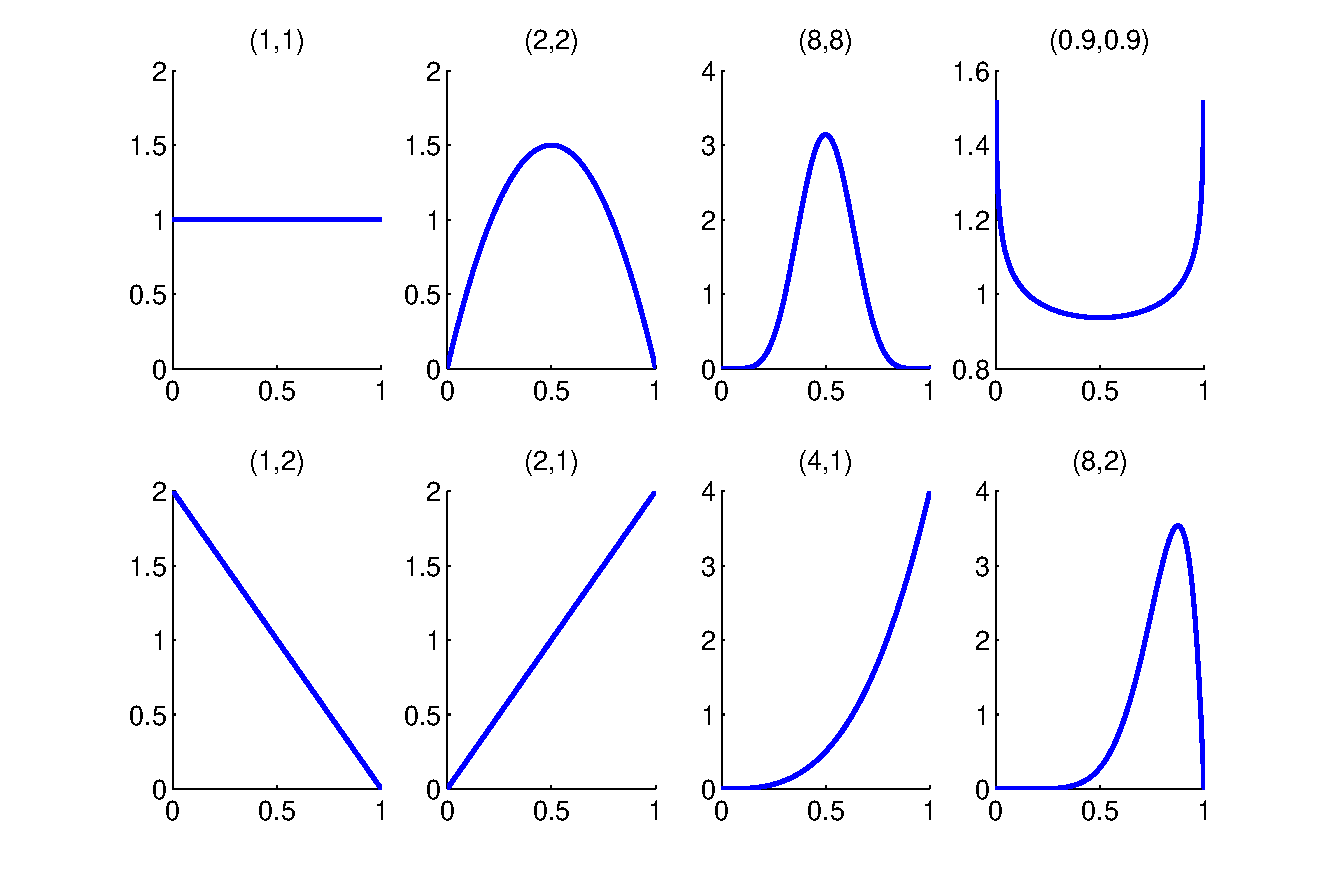
\includegraphics[width=10cm]{BetaZoo}
}

\frame{\frametitle{We will use a beta distribution as a prior for $q$.}
\begin{itemize}
\item 
Beta distribution: 
\begin{align}
\pi(q| \alpha, \alpha_{2})= \frac{1}{Z}q^{\alpha_1-1} (1-q)^{\alpha_{2}-1}
\end{align}
\item \pause Normalizing constant: the 'beta function'
\begin{align}
Z= \int_0^1 q^{\alpha_1-1} (1-q)^{\alpha_{2}-1} dq=: B(\alpha_1, \alpha_{2})
\end{align}
\item \pause Mean and Variance:
\begin{align}
\mbox{E}(q|\alpha_1,\alpha_{2})&= \frac{\alpha_1}{\alpha_1+\alpha_{2}}\\
\mbox{Var}(q|\alpha_1,\alpha_{2})&= \frac{\alpha_1\alpha_{2}}{(\alpha_1+\alpha_{2})^2(\alpha_1+\alpha_{2}+1)}
\end{align}
\item \pause Symmetric case and heuristics:  [on board]
\end{itemize}

}
\frame{\frametitle{Illustration: The posterior gets more peaked as more data is coming in. }

\centering
Data: $D=\{1     1     0     1     1     1     1     1     0\}$

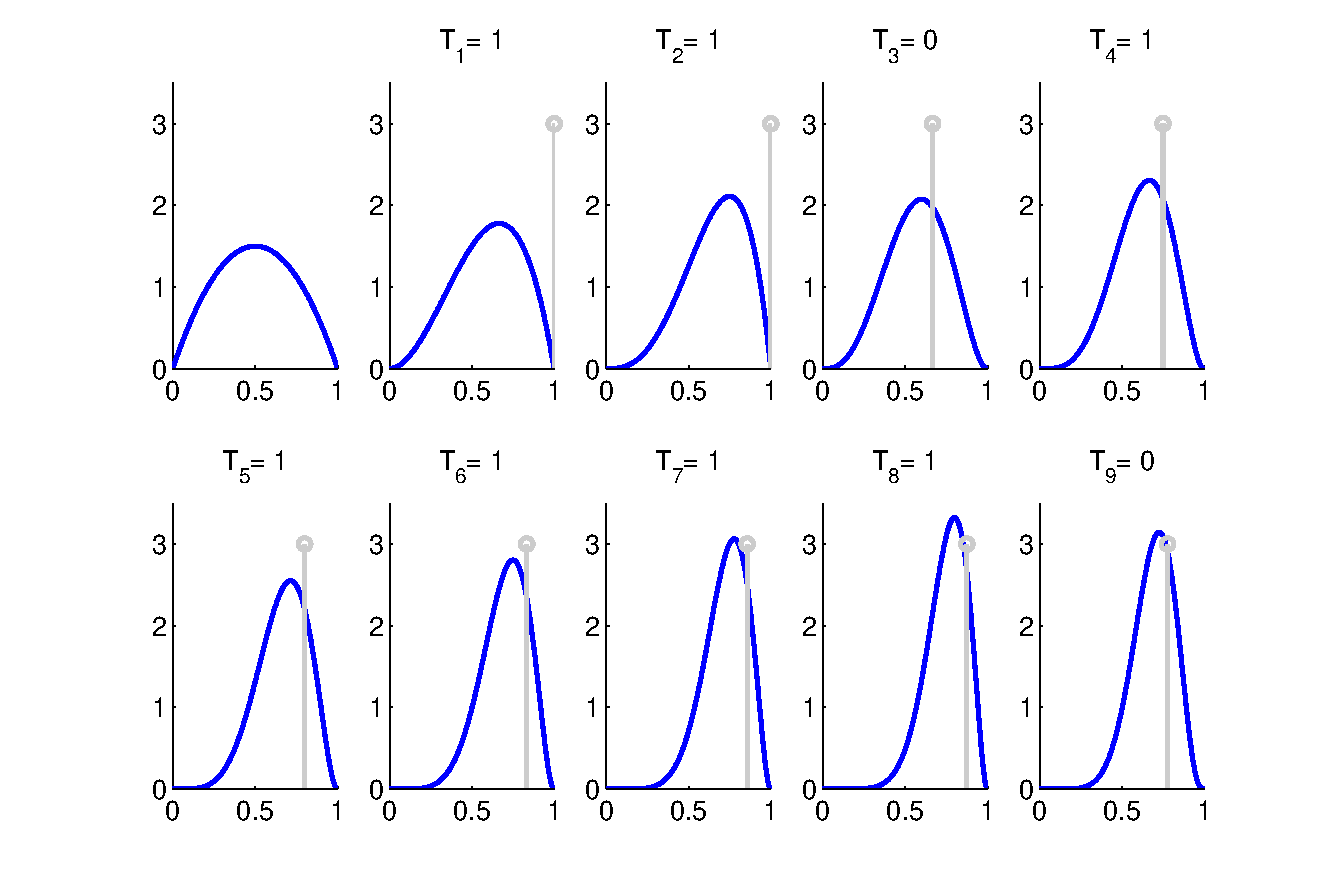
\includegraphics[width=10cm]{BetaPosterior}
}

\frame{\frametitle{The posterior distribution can be calculated in closed form.}

We use $S_n$ to denote the number of heads on the first $n$ trials.
\vspace{.5cm}


 \pause Maximum likelihood estimation:

\vspace{.5cm}

[on board]

\vspace{.5cm}

 \pause Posterior distribution:

\vspace{.5cm}

[on board]

\vspace{.5cm}

\pause We can either take all the data and calculate the posterior at once, or do it sequentially as new data comes in:

\vspace{.5cm}

[on board]
}


\frame[shrink=10]{\frametitle{We can use the posterior distribution for predictions ... }
\vspace{.5cm}
After observing $N$ coin-flips, what is our prediction for the next coin flip?
\begin{align}
P(T^*=1| D)&= \int_0^1 P(T^*=1|q) P(q|D) dq\\
& = \int_0^1 q P(q|D) dq\\
&= \mbox{E}(q|D) \\
&=\frac{\alpha_1+S_N}{(\alpha_1+ S_N)+(\alpha_{2}+N-S_N)}\\
&=\frac{\alpha_1+S_N}{(\alpha_1+\alpha_2+N)}
\end{align}

\pause
\vspace{.5cm}
In our example, $\mbox{E}(q|D)=0.69$, and $\mbox{MLE}=0.78$. 

\pause
\vspace{.5cm}
Q: What happens if $N$ gets very large?

\pause
\vspace{.5cm}
Note: This is a bit of a special case-- in general, the predictive distribution is not simply the likelihood evaluated at the mean!!!
}

\frame{\frametitle{... for statistical reasoning .... }
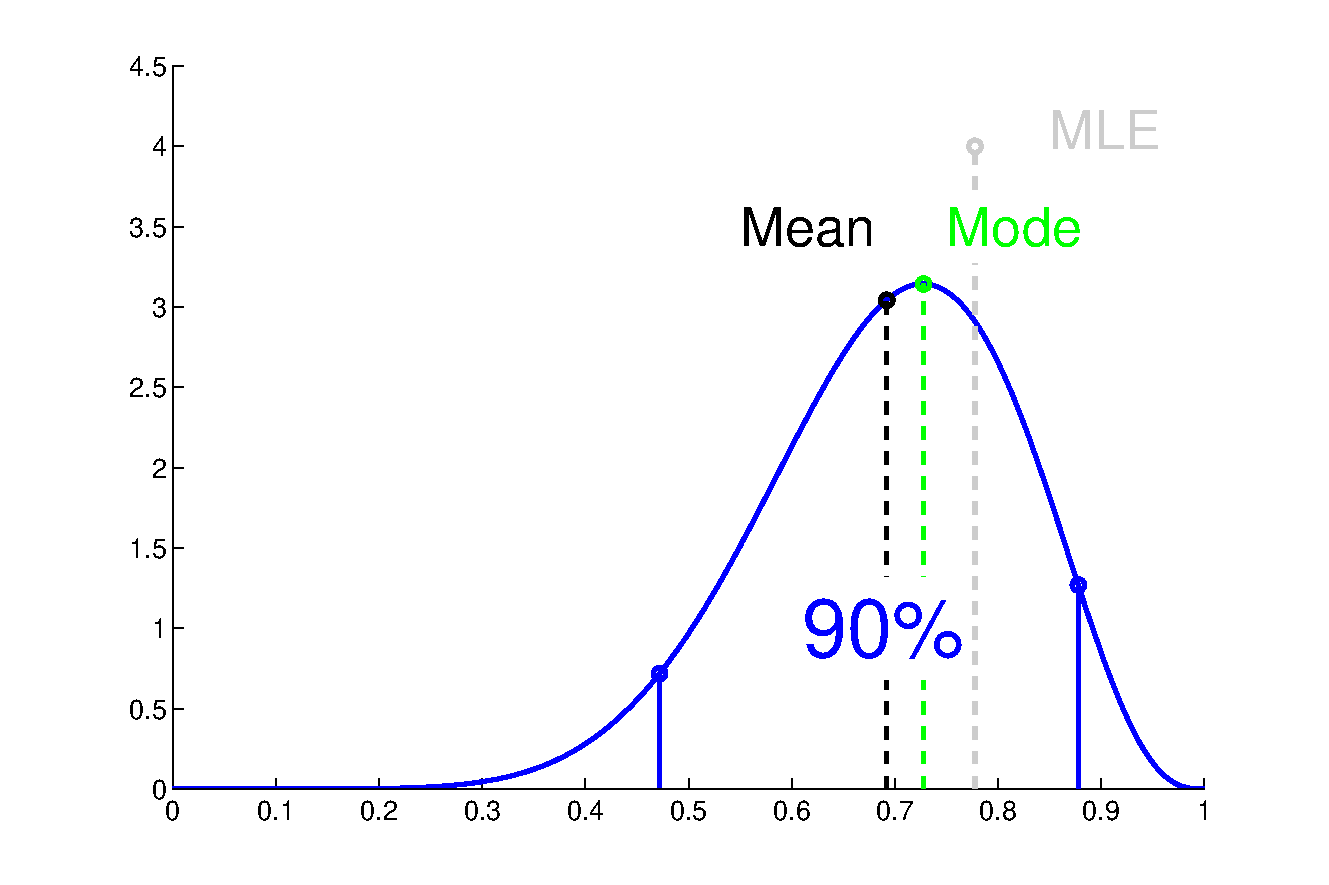
\includegraphics[width=10cm]{BetaPosteriorConfidence}
}


\frame{\frametitle{... and for making decisions. }
Someone offers you the bet that you get 1 euros if you predict the next coin toss correctly, but you have to pay 2 euros if if you are wrong. 

Should you take the bet? What should you predict?

\begin{align}
C(t^*,\hat t)=
\begin{cases}
-1 &\mbox{if~} t^*= \hat t\\
2 &\mbox{if~} t^*\neq \hat t\\
\end{cases}
\end{align}

Expected cost: 
\begin{align}
E(C)=\sum_{t^*=0}^1 C(t^*,\hat t) P(t^*| D)
\end{align}

\pause
If we predict tail ($t^*=0$): 
\begin{align}
E(C)&= P(t^*=1|D) C(0,1)+P(t^*=0|D) C(0,0)  \\
&=0.69 (2)  + 0.31 (-1)= 1.07
\end{align}

\pause
If we predict head ($t^*=1$): 
\begin{align}
E(C)=0.69 (-1)  + 0.31 (2)= -0.07;
\end{align}





}

\section{Conjugate priors and the exponential family}

\frame{\frametitle{Why was inference so easy here?}
\begin{itemize}
\item Posterior distribution had a closed form solution. \pause
\item In fact, the posterior had the same functional form as the prior, just different parameters. \pause
\item Parameters of posterior could be calculated by simply adding observations to prior parameters. \pause
\item We used a likelihood from the \alert{exponential family} and its \alert{conjugate prior}. In this case,  Bayesian inference is always easy. \pause
\item For this reason, exponential families and conjugate priors are used extensively in Bayesian modelling, often as 'building blocks' of more complicated models.
\end{itemize}

}

\frame{\frametitle{Inference is easy whenever the likelihood is in the exponential family and the prior is its conjugate.}
\begin{itemize}
\item Exponential family distributions  have the form 
\begin{align}
P(\xx|\theta)&= g(\theta) f(\xx) \exp\left(\phi(\theta)^\top S(\xx)\right)
\end{align}

\item \pause The conjugate prior is
\begin{align}
\pi(\theta)&= F(\tau,\nu) g(\theta)^\nu \exp(\phi(\theta)^\top \tau)
\end{align}
\item \pause  Calculating the posterior:
\begin{align}
 [\mbox{on board}]
\end{align}
\end{itemize}

}
 
\frame{\frametitle{Inference is easy whenever the likelihood is in the exponential family and the prior is its conjugate.}
The posterior given an exponential family likelihood and conjugate prior is 
\begin{align}
P(\theta|D)= F(\tau+ \sum_i S(x_i), \nu+N) g(\theta)^{\nu+N} \exp\left(\phi(\theta)^\top(\tau +\sum_i S(x_i)    )\right)
\end{align}
\pause
\begin{itemize}
\item $\phi(\theta)$ is the vector of \alert{natural parameters}
\item $\sum_i S(x_i)$ is the vector of \alert{sufficient statistics}
\item $\tau$ are \alert{pseudo-observations}
\item $\nu$ is the scale of the prior\\
\end{itemize}

\pause
The exponential family includes most common distributions, including the Normal, Exponential, Gamma, Chi-square, Beta, Dirichlet, Bernoulli, Poisson, Wishart and the Inverse Wishart.
}
  
  \frame{\frametitle{How can we put our coin-example into this framework?}
  [on board]
  }
  
  
%\subsection{Lists I}
%\begin{itemize}
%\item Introduction to  \LaTeX  
%\item Course 2 
%\item Termpapers and presentations with \LaTeX 
%\item Beamer class
%\end{itemize} 

%\frame{\frametitle{lists with pause}
%\begin{itemize}
%\item Introduction to  \LaTeX \pause 
%\item Course 2 \pause 
%\item Termpapers and presentations with \LaTeX \pause 
%\item Beamer class
%\end{itemize} 
%}

%\subsection{Lists II}
%\frame{\frametitle{numbered lists}
%\begin{enumerate}
%\item Introduction to  \LaTeX  
%\item Course 2 
%\item Termpapers and presentations with \LaTeX 
%\item Beamer class
%\end{enumerate}
%}
%\frame{\frametitle{numbered lists with pause}
%\begin{enumerate}
%\item Introduction to  \LaTeX \pause 
%\item Course 2 \pause 
%\item Termpapers and presentations with \LaTeX \pause 
%\item Beamer class
%\end{enumerate}
%}

%\section{The Normal distribution} 
%\subsection{Tables}
%\frame{\frametitle{Next week}

%Gaussians

%\vspace{1cm}
%Gaussians


%\vspace{1cm}
%Linear Regression

%}


%\frame{\frametitle{The multivariate Gaussian}
%}
%\begin{tabular}{|c|c|c|}
%\hline
%\textbf{Date} & \textbf{Instructor} & \textbf{Title} \\
%\hline
%WS 04/05 & Sascha Frank & First steps with  \LaTeX  \\
%\hline
%SS 05 & Sascha Frank & \LaTeX \ Course serial \\
%\hline
%\end{tabular}}
%}

%\frame{\frametitle{Tables}
%}
%\frame{\frametitle{Tables with pause}
%\begin{tabular}{c c c}
%A & B & C \\ 
%\pause 
%1 & 2 & 3 \\  
%\pause 
%A & B & C \\ 
%\end{tabular} }


%\section{Section no. 4}
%\subsection{blocs}
%\frame{\frametitle{blocs}

%\begin{block}{title of the bloc}
%bloc text
%\end{block}

%\begin{exampleblock}{title of the bloc}
%bloc text
%\end{exampleblock}


%\begin{alertblock}{title of the bloc}
%bloc text
%\end{alertblock}
%}
\end{document}

